%%%%%%%%%%%%%%%%%%%%%%%%%%%%%%%%%%%%%%%%%%%%%%%%%%%%%%%%%%%%%%%%%%%%%%%%%%%%%%%

\chapter{RESULTADOS PRELIMINARES}\label{ch:impl}

Para a implementação do cubo, é necessário conhecimento sobre o domínio dos dados e como eles estão organizados.
Para esse estágio da pesquisa, foram utilizados dados do SCD-2 fornecidos pelo CCS, porém alguns softwares foram implementados como parte da pesquisa sobre o cubo de dados e como resultados da análise dos dados.

\section{SCD-Dashboard}\label{ch:impl:dash}

Os dados vindos do SCD2 possuem 135 dimensões e estão distribuídos em um período de 25 anos, tornando a sua análise não trivial.
Durante atividades de \textit{Data Science} era necessário criar muitos gráficos e visualizações com períodos e dimensões variadas, e com tantas dimensões isso levava vários pedaços de código copiados para criar relatórios sobre os dados e dimensões.

Para facilitar essa análise e automatizar esse problema, foi criado um software chamado \textbf{SCD-dashboard} para facilitar na visualização dos dados de telemetria.
Ele foi implementado utilizando o pacote Shiny~\cite{changShinyWebApplication2019} da linguagem R~\cite{rcoreteamLanguageEnvironmentStatistical2018}, que já estava sendo utilizada para criar as visualizações, a interface permite apenas criar as visualizações e aplicar os outros algoritmos relacionados de uma interface amigável e sem ter a necessidade de escrever código.

Ele funciona sobre um banco de dados PostgreSQL que possui o histórico das telemetrias já importadas e propriamente transformadas por outro script feito só para os dados do SCD2, porém devem funcionar para qualquer dado exportado via CSV pelo SatCS.

Essa ferramenta também pode ser vista como um piloto para implementar algo semelhante as \textit{dashboards} criadas por outras agências, sendo que tem um precedente na ferramenta MARTE utilizada pela NASA~\cite{fernandezTelemetryAnomalyDetection2017}, que utiliza das mesmas tecnologias e conceitos, porém focada no algoritmo de detecção de anomalias.
Ferramentas mais parecidas, e mais completas, estão no CHART e nas dashboard criadas usando o Kibana em~\cite{mateikUsingBigData2017} e~\cite{zhangBigDataFramework2017}.

\begin{figure}[ht]
	\caption{Aparência do SCD-Dashboard}\label{fig:scddashboard}
	\vspace{6mm}
	\begin{center}
		\resizebox{15cm}{!}{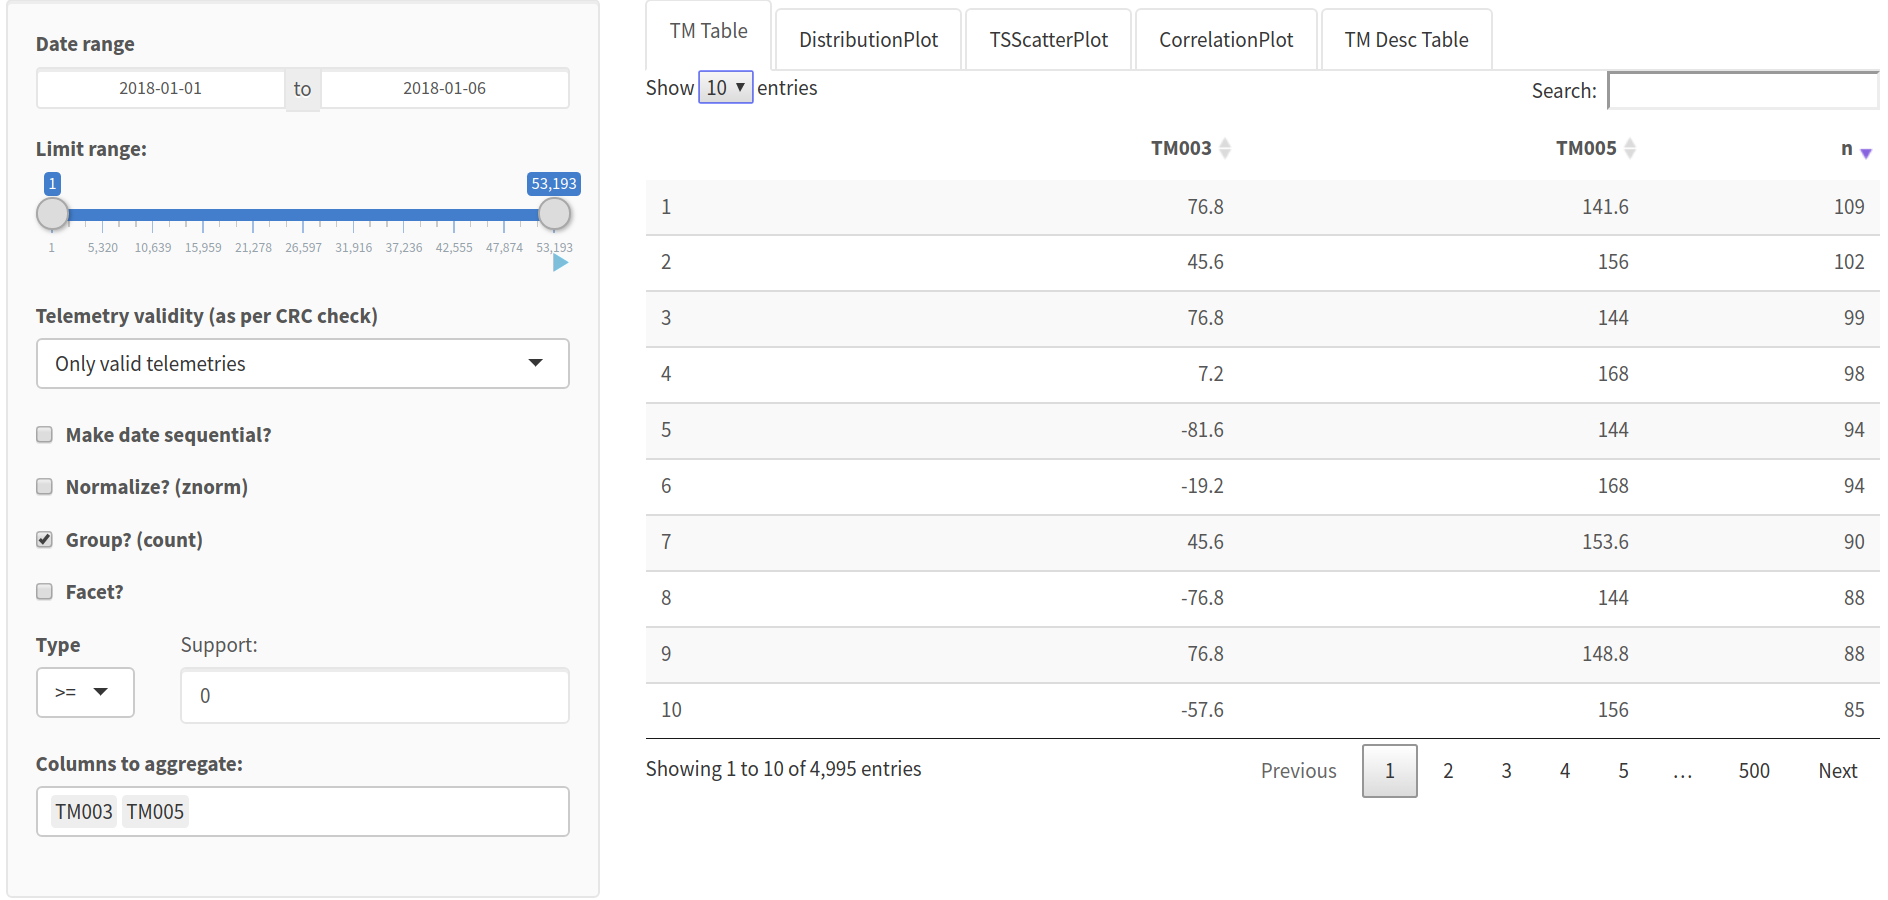
\includegraphics{Figuras/Dashboardview.png}}
	\end{center}
	\vspace{4mm}
	\legenda{}
	\FONTE{Produção do autor.}
\end{figure}

Essa ferramenta foi utilizada extensamente para visualização dos dados e para análise exploratória, sendo que foi melhorada durante as disciplinas de \textit{Data Science} e Algoritmos de \textit{Data Mining}, com apresentações da mesma feitas utilizando ela.

\section{RFragCubing}\label{ch:impl:rfrag}

{\color{cerulean}
O algoritmo \textit{FragCubing}, apresentado na seção~\ref{ch:corr:cube:frag}, foi disponibilizado em forma compilada via código de C++, porém ele não permitia a importação dos dados de telemetria sem um trabalho de pré-processamento não trivial antes.
Como essa implementação foi a utilizada no trabalho de~\cite{silva:2015:abordagensParaCubo}, a implementação possui histórico de uso, portanto o seu uso contínuo seria interessante.
}

Para isso, foi criado um pacote na linguagem R chamado de \textbf{RFragCubing}, que permite a integração com o algoritmo implementado em C++.
Esse pacote faz a interface com o código do \textit{FragCubing}, permitindo importar os dados, executar as queries e retornar os resultados das mesmas, bem como algumas adições de medidação de memória e tempo de processamento.
Uma das vantagens do pacote está na distribuição, com uma interface que permite a execução da mesma consulta em outros algoritmos de construção do cubo, uma das razões para fazer a implementação, para facilitar a comparação entre os algoritmos.

\begin{figure}[ht]
  \caption{Carregando dados de telemetria no \textit{RFragCubing}}\label{fig:shinyrfrag}
	\vspace{6mm}
	\begin{center}
		\resizebox{10.5cm}{!}{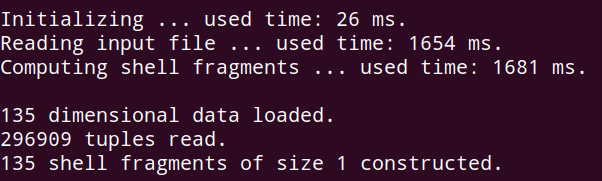
\includegraphics{Figuras/RFragInit.png}}
	\end{center}
	\vspace{4mm}
	\legenda{}
	\FONTE{Produção do autor}
\end{figure}

\section{Medida de Similaridade}\label{ch:impl:similarity}

Utilizando a ferramenta criada em~\ref{ch:impl:dash} para uma atividade de exploração de dados que envolvia realizar consultas multidimensionais baseadas no conceito do cubo de dados, um padrão foi notado entre as telemetrias: quando uma medida de agregação por contagem era executada sobre telemetrias que se sabia ter algum tipo de relacionamento entre elas, elas possuiam uma curva característica, como da figura~\ref{fig:scdsimilaritygraph}.

\begin{figure}[ht]
	\caption{Curva de de agregação gerada pela SCD-Dashboard}\label{fig:scdsimilaritygraph}
	\vspace{6mm}
	\begin{center}
		\resizebox{15cm}{!}{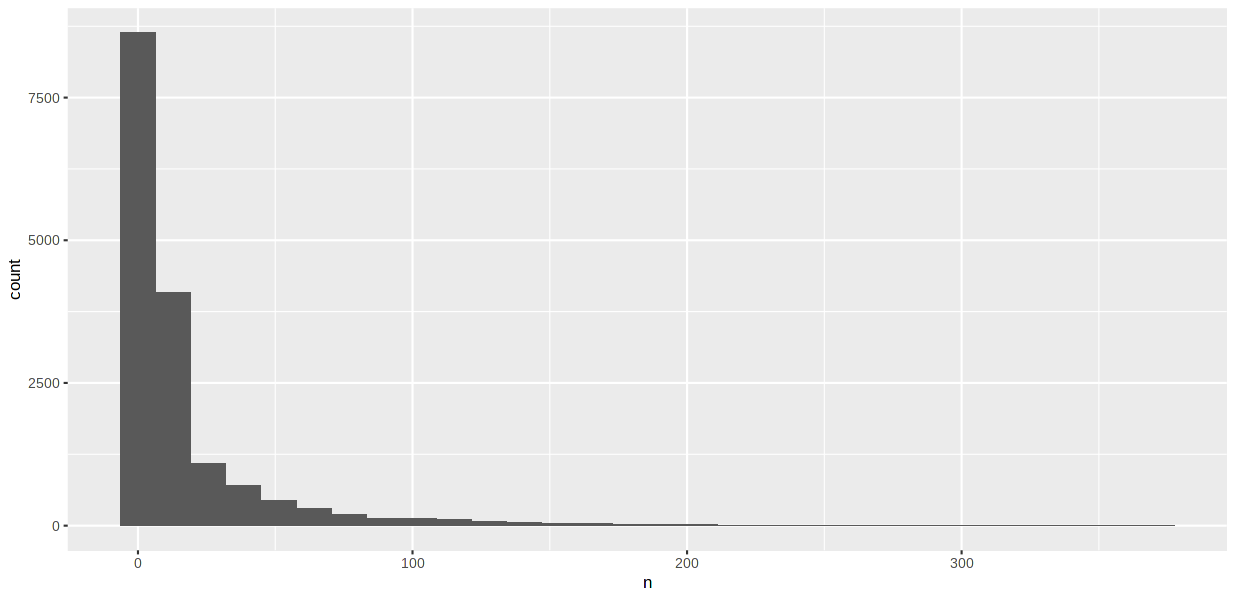
\includegraphics{Figuras/SimilarityCurve.png}}
	\end{center}
	\vspace{4mm}
	\legenda{Agregação de duas telemetrias ao longo de um mês}
	\FONTE{Produção do autor.}
\end{figure}

Essa curva foi utilizada para desenvolver um algoritmo de classificação do relacionamento entre as telemetrias, pois possuia algumas vantagens: a medida de contagem dos valores que se repetem é independente do tipo dos valores em si, permitindo comparar um valor contínuo com um discreto bem como discretos com discretos e contínuos com contínuos, de equipamentos diferentes e com características diferentes; e é uma medida que funciona com qualquer número de dimensões, sendo uma operação $\mathcal{O}(D)$, com $D$ sendo o número de dimensões, tornando a sua integração, e subsequente otimização, com um algoritmo de construção de cubo de dados simplificada.

\begin{figure}[ht]
	\caption{Resultados preliminares da Medição de Relacionamento}
	\vspace{6mm}
	\begin{center}
		\resizebox{15cm}{!}{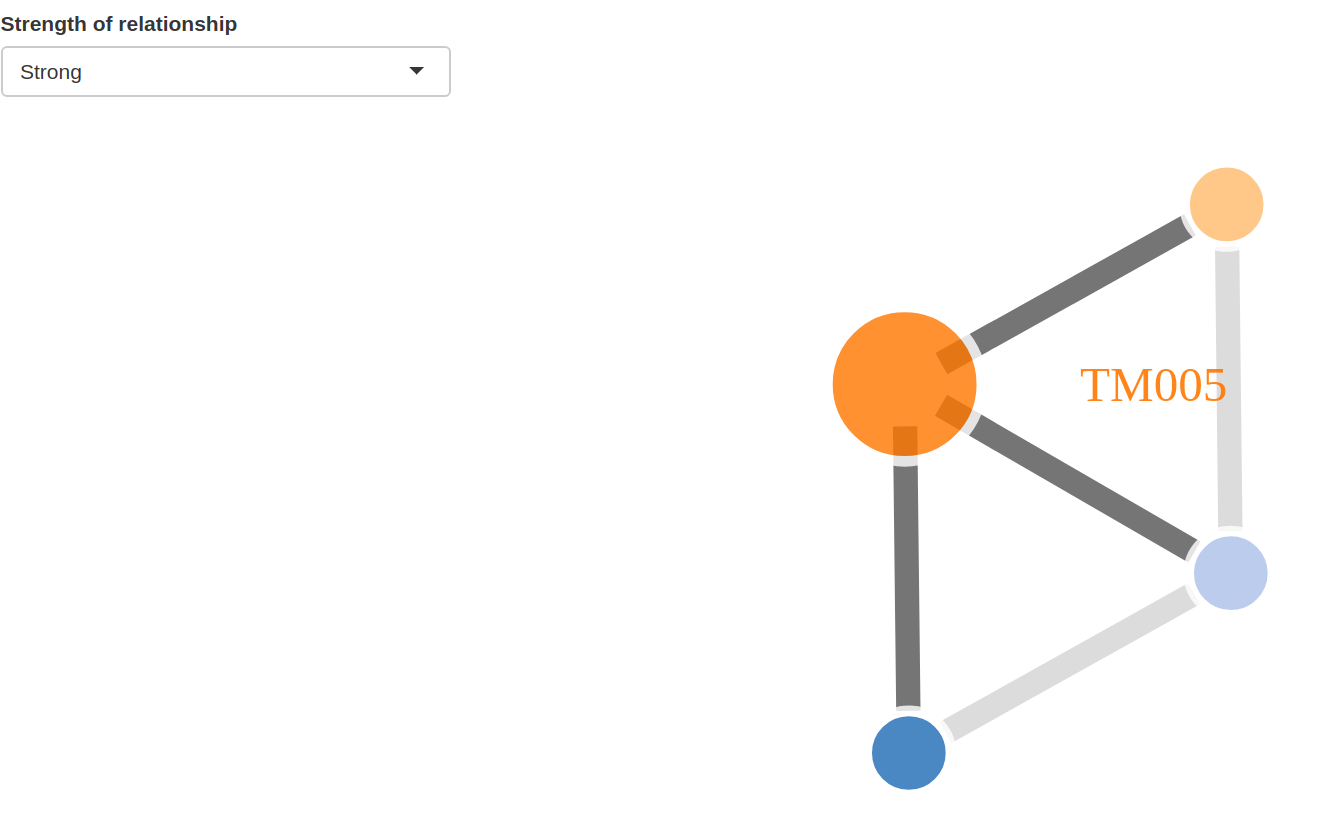
\includegraphics{Figuras/SimilarityGraph.png}}
	\end{center}
	\vspace{4mm}
	\legenda{Um grupo de telemetrias com relacionamento forte}
	\label{fig:similarityresults}
	\FONTE{Produção do autor.}
\end{figure}

O algortimo está sujeito a Maldição de Dimensionalidade explicada na seção~\ref{ch:fun:cube:comp}, pois ele verifica a relação entre um número $n$ de telemetrias definida pelo usuário, tendo $2^D$ possíveis combinações para $D$ dimensões, assim ele atualmente só foi executado para todas as combinações de 2 dimensões dos dados do SCD.
Mesmo assim, e por ser uma operação demorada mesmo com apenas um ano de telemetrias, ainda são $8911$ combinações.
Esse número só cresce com o número de combinações, sendo que a execução de todas as combinações com mais de 4 dimensões é inviável.

O algoritmo está sendo revisado atualmente, mas o objetivo é implementar o resultado no algoritmo de construção do cubo, sendo que as dimensões que tem um relacionamento associado como forte ou média seriam as combinações com maior interesse pelos operadores, pois provavelmente seriam as operações mais comumemente executadas por eles.

Isto também abre espaço para um algoritmo de detecção de anomalias: caso durante uma passagem um relacionamento que antes era tido como forte muda para um relacionamento fraco ou perde o relacionamento, isso pode ser um sinal de que alguma coisa está de errado com esse grupo de telemetrias.
Isso pode ajudar no conhecimento dos operadores, pois os relacionamentos entre grupos de telemetrias são difíceis de serem visualizados e apenas os operadores com mais experiência em um dado satélite conseguem visualizar alguns desses relacionamentos.

Existem alguns trabalhos de visualização dos relacionamentos, porém estes geralmente utilizam algoritmos de indução de regras, cuja saída é de difícil interpretação, como demonstrado em~\cite{kannanMiningSatelliteTelemetry2016}.
A abordagem aqui proposta tem potencial de ter respostas mais relevantes para os operadores, porém precisa ser avaliada por um operador ainda, um dos próximos passos deste trabalho.

